\documentclass[transacties.tex]{subfiles}
\begin{document}

\chapter{Voorbeeld}

\section{Is dit transactierooster herstelbaar?}
\subsection*{Opgave}
\begin{figure}[H]
\centering
\begin{tabular}{c|c|c}
$T_1$ & $T_2$ & $T_3$\\
\hline
read(A) &&\\
&read(A)&\\
&&read(A)\\
read(B)&&\\
&write(A)&\\
&&read(B)\\
&&write(B)\\
write(B)&&\\
&commit&\\
&&commit\\
commit&&\\
\end{tabular}
\end{figure}


\subsection*{Antwoord}
\subsubsection*{Schrijven}
\begin{itemize}
\item $T_2$ schrijft naar $A$.
\item $T_1$ en $T_3$ schrijven naar $B$.
\end{itemize}
\subsubsection*{Lezen}
\begin{itemize}
\item $T_1$,$T_2$ en $T_3$ lezen van $A$ 
\item $T_1$ en $T_3$ lezen van $B$
\end{itemize}
\subsubsection*{Checks}
\begin{itemize}
\item $T_1$:
\begin{itemize}
\item $T_2$ schrijft naar $A$ en $T_1$ leest $A$\\
$T_2$ moet v\'o\'or $T_1$ comitten. $\rightarrow$ OK
\item $T_3$ schrijft naar $B$ en $T_1$ leest $B$.\\
$T_3$ moet v\'o\'or $T_1$ comitten. $\rightarrow$ OK
\end{itemize}

\item $T_2$ leest van $A$ maar geen andere transactie schrijft naar $A$. $\rightarrow$ OK

\item $T_3$
\begin{itemize}
\item $T_1$ schrijft naar $B$ en $T_3$ leest $B$.\\
$T_1$ moet v\'o\'or $T_3$ comitten. $\rightarrow$ NOK
\item $T_2$ schrijft naar $A$ en $T_3$ leest $A$.\\
$T_2$ moet v\'o\'or $T_3$ comitten. $\rightarrow$ OK
\end{itemize}
\end{itemize}
\subsubsection*{Conclusie}
\'E\'en van de tests slaagde niet. Dit rooster is dus niet herstelbaar. Het rooster is bijgevolg ook niet cascadeloos of strict.

\section{Is dit transactierooster conflict-serialiseerbaar?}
\subsection*{Opgave}
Gegeven volgend transactierooster $S$. Bepaal of $S$ conflict-serialiseerbaar is.
\begin{figure}[H]
\centering
\begin{tabular}{c|c|c}
$T_1$ & $T_2$ & $T_3$\\
\hline
&&read(B)\\
&&read(C)\\
read(A)&&\\
write(A)&&\\
&&write(B)\\
&&write(C)\\
&read(C)&\\
read(B)&&\\
write(B)&&\\
&read(Y)&\\
&write(Y)&\\
&read(A)&\\
&write(A)&\\
\end{tabular}
\end{figure}
\subsection*{Antwoord}
\subsubsection*{Precedence-graaf}
We stellen volgende graaf op.
\begin{figure}[H]
\centering
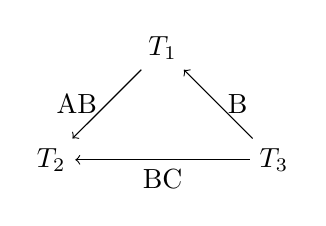
\begin{tikzpicture}
[align=center,node distance=2cm]
 \node (T1) {$T_1$};
 \node (T2) [below left of=T1] {$T_2$};
 \node (T3) [below right of=T1]{$T_3$};
 
 \draw (T1) edge[->] node [left] {AB} (T2);
 \draw (T3) edge[->] node [below] {BC} (T2);
 \draw (T3) edge[->] node [right] {B}  (T1);
 	
\end{tikzpicture}
\end{figure}
\subsubsection*{Conclusie}
De precedence-graaf is acyclisch. $S$ is dus conflict-serialiseerbaar. Het equivalente seriele rooster bekomen we door $T_3$, $T_1$ en $T_2$ in die volgorde af te gaan.

% Examenvraag
\section{Bespreek dit transactierooster}
\subsection*{Opgave}
Is dit transactierooster $S$ herstelbaar, cascadeloos, strikt, serieel, conflict-serializeerbaar?
\begin{figure}[H]
\centering
\begin{tabular}{c|c}
\multicolumn{2}{c}{Niet strict}\\
$T_1$&$T_2$\\
\hline
read(A) &\\
& read(A)\\
read(B)&\\
write(B)&\\
&write(A)\\
&commit\\
commit&
\end{tabular}
\end{figure}
\subsection*{Antwoord}
\subsubsection*{Herstelbaarheid}
Schrijven
\begin{itemize}
\item $T_1$ en $T_2$ schrijven naar $A$.
\item $T_1$ schrijft naar $B$.
\end{itemize}
Lezen
\begin{itemize}
\item $T_2$ schrijft naar $A$.
\item $T_1$ schrijft naar $B$.
\end{itemize}
Checks
\begin{itemize}
\item $T_2$ schrijft naar $A$ en $T_1$ leest $A$.\\
$T_2$ moet v\'o\'or $T_1$ comitten $\rightarrow$ OK.
\item $T_1$ schrijft naar $B$ maar er is geen andere transactie die $B$ leest. $\rightarrow$ OK.
\end{itemize}
$S$ is dus herstelbaar.
\subsubsection*{Cascadeloosheid}
$S$ is cascadeloos. $T_1$ en $T_2$ schrijven nooit naar een gemeenschappelijke waarde.

\subsubsection*{Striktheid}
$S$ is strict. $T_1$ leest uit $A$ v\'o\'or $T_2$ naar $A$ schrijft.

\subsubsection*{Serieel en conflict-serializeerbaarheid}
$S$ is niet serieel. De operaties gebeuren duidelijk door elkaar.
Om conflict-serializeerbaarheid te testen stellen we de volgende graaf op.
\begin{figure}[H]
\centering
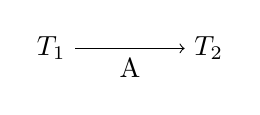
\begin{tikzpicture}
[align=center,node distance=2cm]
 \node (T1) {$T_1$};
 \node (T2) [right of=T1] {$T_2$};
 
 \draw (T1) edge[->] node [below] {A} (T2);
\end{tikzpicture}
\end{figure}
Deze graaf is duidelijk acyclisch. $S$ is dus serialiseerbaar. $S$ is bovendien conflict-equivalent met $S'$ waarbij $S'$ $T_1$ en $T_2$ in die volgorde appart afhandelt.

% Examenvraag
\section{Timestamp ordering}
\subsection*{Opgave}

\subsection*{Antwoord}


\end{document}
